\setcounter{step}{0}

\subsection{ Pudingová torta }

\begin{ingredient}
  
      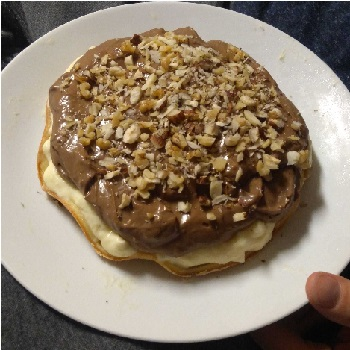
\includegraphics[height=5.5cm]{images/eh_torta}
  
  \def\portions{  }
  \textbf{ {\normalsize Ingrediencie (4 porcie):} }

  \begin{main}
      \item 
  \end{main}
  
    \begin{subingredient}{Piškótové cesto}
        \item 200g kryštálový cukor
        \item 1dl voda
        \item 4ks vajce
        \item 1dl olej (???)
        \item 200g hladká múka
        \item 1ks vanilkový cukor
        \item 1ks prášok do pečiva
    \end{subingredient}
  
    \begin{subingredient}{Pudingy}
        \item 500ml mlieka
        \item puding
        \item 2PL cukru
    \end{subingredient}
  
\end{ingredient}
\begin{recipe}
\textbf{ {\normalsize Príprava:} }
\begin{enumerate}

  \item{Urobíme piškótové cesto: }
      \begin{enumerate}
          \item{Žĺtka vymiešame s cukrami do peny}
          \item{Pridáme olej a vodu a premiešame}
          \item{Pridáme múku s práškom do pečiva}
          \item{Pridáme sneh z bielok}
          \item{Pečieme 20 minút na 180°C}\end{enumerate}
  \item{Urobíme puding a vykydneme na piškót}
  \item{Pred podávaním necháme vychladiť v chladničke}

\end{enumerate}
\end{recipe}

\begin{notes}
  
\end{notes}	
\clearpage
